\documentclass[tikz]{standalone}

\usepackage[latin1]{inputenc}
\usepackage{tikz}

% GNUPL
\begin{document}

\usetikzlibrary{decorations.pathreplacing,decorations.markings,arrows}
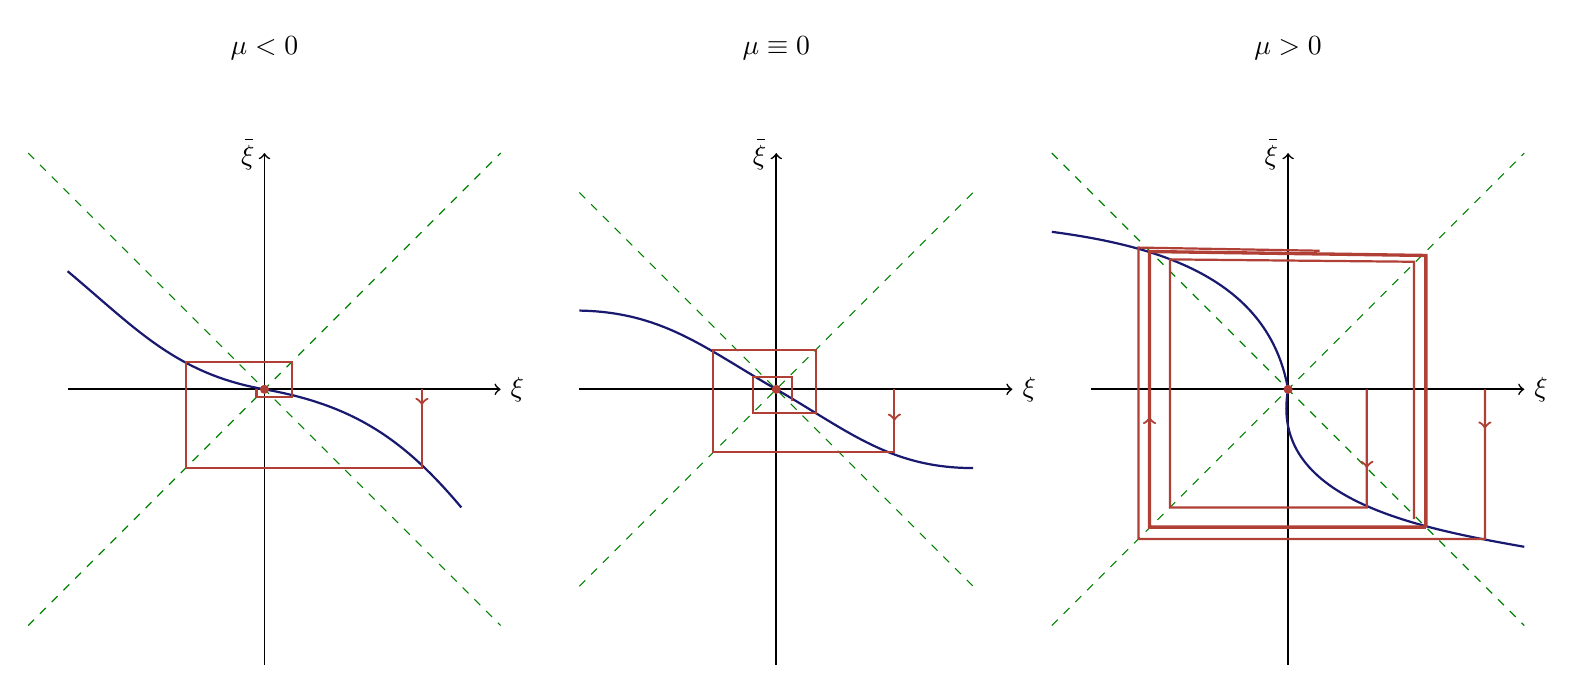
\begin{tikzpicture}
    %\mu<0
    \coordinate [label=-90:$\mu<0$] (8) at (3,8.6);

    \draw[semithick] [->] (0.5,4) -- (6,4) node[right] {$\xi$};
    \draw[semithick] [->] (3,0.5) -- (3,7) node[left] {$\stackrel{\_}{\xi}$};
    % \draw [black, semithick, domain=0:6,samples=200] plot (\x,  {1+0.2*(\x)^2+0.05*(\x)});
    \draw [color={rgb,255:red,25; green,25; blue,112},thick] (0.5,5.5) to [out=-40,in=170] (3,4) to [out=-10,in=130] (5.5,2.5);
    \draw [black, dashed, color={rgb,255:red,0; green,128; blue,0},] (0,7) -- (6, 1);
    \draw [black, dashed, color={rgb,255:red,0; green,128; blue,0},] (0,1) -- (6, 7);
    \draw [color={rgb,255:red,176; green,63; blue,53},thick] [->] (5,4) -- (5,3.8);
    \draw [color={rgb,255:red,176; green,63; blue,53},thick] (5,4) -- (5,3) --(2,3) -- (2,4.35) -- (3.35,4.35) -- (3.35,3.9) -- (2.9,3.9) -- (2.9,4);
    \draw [fill,color={rgb,255:red,176; green,63; blue,53}] (3,4) circle [radius=0.05];
	%\mu=0
    \coordinate [label=-90:$\mu \equiv0$] (8) at (9.5,8.6);

    \draw[semithick] [->] (7,4) -- (12.5,4) node[right] {$\xi$};
    \draw[semithick] [->] (9.5,0.5) -- (9.5,7) node[left] {$\stackrel{\_}{\xi}$};
    \draw [black, dashed, color={rgb,255:red,0; green,128; blue,0},] (7,1.5) -- (12, 6.5);
    \draw [black, dashed, color={rgb,255:red,0; green,128; blue,0},] (7,6.5) -- (12, 1.5);
    \draw [color={rgb,255:red,25; green,25; blue,112},thick] (7, 5) to [out=-1,in=150] (9.5,4) to [out=-30,in=180] (12,3);
    \draw [color={rgb,255:red,176; green,63; blue,53},thick] [->] (11,4) -- (11,3.6);
    \draw [color={rgb,255:red,176; green,63; blue,53},thick] (11,4) -- (11,3.2) --(8.7,3.2) -- (8.7,4.5) --(10,4.5) -- (10,3.7) --(9.2,3.7) --(9.2,4.16) -- (9.7,4.16) --(9.7,3.85);
    \draw [fill,color={rgb,255:red,176; green,63; blue,53}] (9.5,4) circle [radius=0.05];
    %\mu>0
    \coordinate [label=-90:$\mu>0$] (8) at (16,8.6);

    \draw[semithick] [->] (13.5,4) -- (19,4) node[right] {$\xi$};
    \draw[semithick] [->] (16,0.5) -- (16,7) node[left] {$\stackrel{\_}{\xi}$};
    \draw [black, dashed, color={rgb,255:red,0; green,128; blue,0},] (13,1) -- (19, 7);
    \draw [black, dashed, color={rgb,255:red,0; green,128; blue,0},] (13,7) -- (19, 1);
    \draw [color={rgb,255:red,25; green,25; blue,112},thick] (13, 6) to [out=-7.5,in=100] (16,4) to [out=-100,in=-190] (19,2);

    \draw [color={rgb,255:red,176; green,63; blue,53},thick] [->] (18.5,3.8) -- (18.5,3.5);
    \draw [color={rgb,255:red,176; green,63; blue,53},thick] (18.5,4) -- (18.5,2.1)--(14.1,2.1) --(14.1,5.8) -- (16.4,5.76);
    \draw [color={rgb,255:red,176; green,63; blue,53},very thick] (17.75,2.25) -- (14.24,2.25)--(14.24,5.75) --(17.75,5.7) --(17.75,2.25);
    \draw [color={rgb,255:red,176; green,63; blue,53},thick] (17,4) -- (17,2.5)--(14.5,2.5) --(14.5,5.65) --(17.6,5.62) -- (17.6,2.35);
    \draw [color={rgb,255:red,176; green,63; blue,53},thick] [->](17,3.5) -- (17,3);
    \draw [color={rgb,255:red,176; green,63; blue,53},thick] [->] (14.24,3.5) --(14.24,3.65);
    \draw [fill,color={rgb,255:red,176; green,63; blue,53}] (16,4) circle [radius=0.05];
\end{tikzpicture}


\end{document}